% fig_87b_mg_sensitivity.tex
% TR-41: 87B sensitivity comparison — SG vs IBR microgrid
%
% Bar chart comparing minimum detectable fault current [pu] for:
%   87L (line differential)       : k_min = 0.0600 pu
%   87B standard (SG)            : k_min = 0.0500 pu  (I_diff_min=0.05 for SG)
%   87B-MG IBR (this report)     : k_min = 0.1176 pu
%   OC adaptive (TR-40 Group 2)  : k_min = 0.0075 pu
%   67Q (GFM fleet)              : k_min = 0.1000 pu

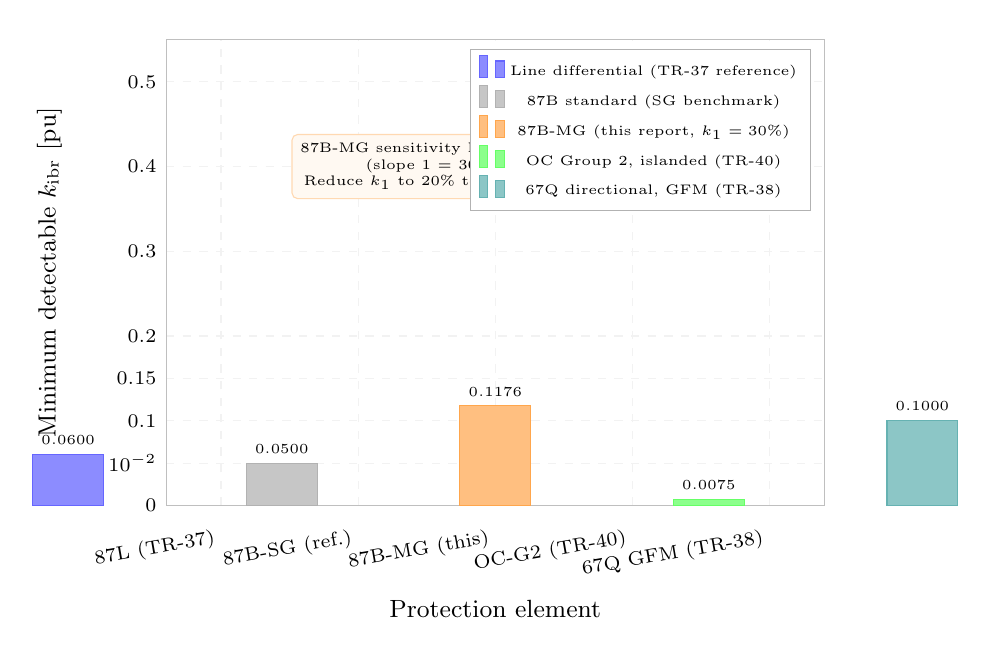
\begin{tikzpicture}
\begin{axis}[
  name         = sensax,
  width        = 0.82\textwidth,
  height       = 7.5cm,
  ybar,
  bar width    = 0.90cm,
  xlabel       = {Protection element},
  ylabel       = {Minimum detectable $k_\mathrm{ibr}$ [pu]},
  xlabel style = {font=\small},
  ylabel style = {font=\small},
  ymin=0, ymax=0.55,
  ytick        = {0,0.05,0.10,0.15,0.20,0.30,0.40,0.50},
  yticklabel style={font=\scriptsize},
  xtick        = {1,2,3,4,5},
  xticklabels  = {87L (TR-37),
                  87B-SG (ref.),
                  87B-MG (this),
                  OC-G2 (TR-40),
                  67Q GFM (TR-38)},
  xticklabel style={font=\scriptsize, rotate=10, anchor=north east},
  tick style   = {draw=none},
  axis line style={gray!50},
  grid         = major,
  grid style   = {gray!10, dashed},
  nodes near coords,
  nodes near coords style={font=\tiny, anchor=south},
  every node near coord/.append style={
    /pgf/number format/.cd, fixed, fixed zerofill, precision=4
  },
  legend style={at={(0.98,0.98)}, anchor=north east, font=\tiny,
                draw=gray!60, fill=white},
  clip=false,
]

%% Bars — colour by performance
% 87L: reference (blue)
\addplot[fill=blue!45, draw=blue!60]
  coordinates {(1, 0.0600)};
\addlegendentry{Line differential (TR-37 reference)}

% 87B-SG: benchmark (gray)
\addplot[fill=gray!45, draw=gray!60]
  coordinates {(2, 0.0500)};
\addlegendentry{87B standard (SG benchmark)}

% 87B-MG: this report (orange — less sensitive due to slope constraint)
\addplot[fill=orange!50, draw=orange!70]
  coordinates {(3, 0.1176)};
\addlegendentry{87B-MG (this report, $k_1=30\%$)}

% OC-G2: most sensitive (green)
\addplot[fill=green!45, draw=green!60]
  coordinates {(4, 0.0075)};
\addlegendentry{OC Group~2, islanded (TR-40)}

% 67Q GFM: less sensitive (teal)
\addplot[fill=teal!45, draw=teal!60]
  coordinates {(5, 0.1000)};
\addlegendentry{67Q directional, GFM (TR-38)}

%% Threshold note
\node[draw=orange!30, fill=orange!5, rounded corners=2pt,
      font=\tiny, inner sep=3pt, align=center]
  at (axis cs:3, 0.40)
  {87B-MG sensitivity limited by slope constraint\\
   (slope 1 = 30\% from Study C).\\
   Reduce $k_1$ to 20\% to reach $k_\mathrm{min}=0.1053$\,pu.};

\end{axis}
\end{tikzpicture}
